\documentclass[letterpaper,11pt]{article}
\oddsidemargin -1.0cm \textwidth 17.5cm

\usepackage[utf8]{inputenc}
\usepackage[activeacute,spanish]{babel}
\usepackage{amsfonts,setspace}
\usepackage{amsmath}
\usepackage{amssymb, amsmath, amsthm}
\usepackage{comment}
\usepackage{float}
\usepackage{amssymb}
\usepackage{dsfont}
\usepackage{anysize}
\usepackage{multicol}
\usepackage{enumerate}
\usepackage{graphicx}
\usepackage[left=1.5cm,top=1.5cm,right=1.5cm, bottom=1.7cm]{geometry}
\setlength\headheight{1.5em} 
\usepackage{fancyhdr}
\usepackage{multicol}
\usepackage{hyperref}
\usepackage{wrapfig}
\usepackage{subcaption}
\pagestyle{fancy}
\fancyhf{}
\renewcommand{\labelenumi}{\normalsize\bfseries P\arabic{enumi}.}
\renewcommand{\labelenumii}{\normalsize\bfseries (\alph{enumii})}
\renewcommand{\labelenumiii}{\normalsize\bfseries \roman{enumiii})}

\begin{document}

\fancyhead[L]{\itshape{Facultad de Ciencias F\'isicas y Matem\'aticas}}
\fancyhead[R]{\itshape{Universidad de Chile}}

\begin{minipage}{11.5cm}
    \begin{flushleft}
        \hspace*{-0.6cm}\textbf{FI1100-6 Introducción a la Física Moderna}\\
        \hspace*{-0.6cm}\textbf{Profesor:} Diego Mardones\\
        \hspace*{-0.6cm}\textbf{Auxiliares:} Gabriel O\textsc{\char13}Ryan, Camila Sepúlveda, Alejandro Silva\\
        \hspace*{-0.6cm}\textbf{Ayudante:} Sebastián Vargas
    \end{flushleft}
\end{minipage}

\begin{picture}(2,3)
    \put(366, 10){
\includegraphics[scale=0.9]{Imágenes/logo/dfi-fcfm.pdf}}
\end{picture}

\begin{center}
	\LARGE\textbf{Auxiliar \#2}\\
	\Large{Movimiento Armónico Simple y Amortiguado}
\end{center}

\vspace{-1cm}
\begin{enumerate}\setlength{\itemsep}{0.4cm}

\rfoot[]{pág. \thepage}

\item[]

\item Un péndulo de 1 $m$ de longitud se suelta desde un ángulo inicial de 15$^\circ$. Después de 1000 $s$, debido a la fricción la amplitud máxima que esta alcanzando el péndulo es 5,5°$^\circ$.

a) A partir de la segunda ley de Newton, plantee la ecuación diferencial que debe satisfacer el movimiento del péndulo.

b) Utiliando una solución de la forma $x(t)=A*e^-^b^t^/^2^m*cos(w*t+\phi)$ ¿Cual es el valor de $b/(2m)$?

c) ¿Cual es la frecuencia angular de oscilación del sistema?

\begin{figure}[h!]
        \centering
        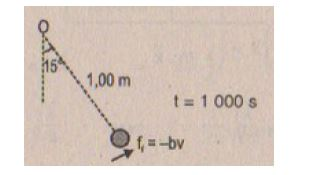
\includegraphics[scale=1
        ]{Imágenes/aux2/3}
    \end{figure}
\end{enumerate}
\end{document}